\documentclass[oneside]{book}
\usepackage{glossaries}
\usepackage{derivative}
\usepackage{pgfplots}
\usepackage{float}
\usepackage{tikz}
\usepackage{circuitikz}
\usepackage{amsmath}
\usepackage{booktabs}
\usepackage{fancyhdr}
\usepackage{amssymb}
\usepackage{amsmath}
\usepackage{subcaption}
\usepackage{lastpage}
\usepackage{array}
\usepackage[hidelinks]{hyperref}
\usepackage{bodegraph}
\usepackage{calc}
\usepackage[a4paper,
    left=10mm,
    right=10mm,
    top=12mm,
    bottom=12mm,
]{geometry}
\setcounter{tocdepth}{3}
\newcolumntype{P}[1]{>{\centering\arraybackslash}p{#1}}
\begin{document}
\pagestyle{fancy}
    \fancyhf{}
\fancyhead[L]{EGB120 Foundations of Electrical Engineering}
\fancyhead[R]{\nouppercase{\leftmark}}
\fancyfoot[L]{Dinal Atapattu}
\renewcommand{\footrulewidth}{0.4pt}
\fancyfoot[R]{Page \thepage\ of \pageref{LastPage}}
    \title{
            Queensland University of Technology\\
            \rule{\linewidth}{0.5pt}
        \centering
        \textbf{EGB120} \\
        Practice Exam Solutions\\
        \vspace{0.4cm}
        \rule{\linewidth}{1.5pt}
        \small{\textit{Professor Geoff Walker}}
    }
    \author{Dinal Atapattu}
    \date{\today}
    \maketitle
    \thispagestyle{empty}
    \tableofcontents
    \chapter{Practice Exam 1}
    Cyril the Circuit Analyst is examining the interaction of both AC and DC sources with a circuit.
    The circuit is drawn below. Pay careful attention to the arrows on the switches which show
    which are initially open, and which are initially closed. Assume that the capacitor is initially
    discharged at t = 0. All times are in seconds.
    \begin{figure}[H]
        \centering
        \begin{circuitikz}[american]
            \draw (0,0)
                to [current source, i=10mA] (0,2)
                to [switch, l=$\text{t=0s}$] (1,2)
                to [opening switch, l=$\text{t=1s}$] (3,2)
                to [switch, l=$\text{t=2s}$] (5,2)
                to [switch, l=$\text{t=5s}$] (7,2)
                to [inductor, l=100$\mu$F] (9,2)
                to [sinusoidal voltage source, v=$10\cos(\omega t)$] (9,0)
                to [short] (0,0);
            \draw (3,2)
                to [capacitor, l=50$\mu$F] (3,0) node[ground] {};
            \draw (5,2)
                to [resistor, l=400$\Omega$] (5,0);
        \end{circuitikz}
    \end{figure}
    \begin{enumerate}
        \item At t = 0, the first switch closes connecting the current source to the capacitor. Find the
        voltage on the capacitor at t = 1 second\\
        \textbf{Solution:}\\
        \begin{minipage}{0.4\linewidth}
            \begin{figure}[H]
                \centering
                \begin{circuitikz}[american]
                    \draw (0,0)
                        to [current source, i=10mA] (0,2)
                        to [short] (2,2)
                        to [capacitor, l=50$\mu$F] (2,0)
                        to [short] (0,0);
                \end{circuitikz}
            \end{figure}
        \end{minipage}
        \begin{minipage}{0.5\linewidth}
            \begin{flalign*}
                v(t) &= \frac{1}{C} \int^{t}_{0} i(\tau)\ d\tau + v(0)\\
                &= \frac{1}{50\times 10^{-6}} \int^{1}_{0} 10\times 10^{-3}\ d\tau + 0\\
                &= 200\text{V}
            \end{flalign*}
        \end{minipage}
        \item At t = 1, the second switch opens disconnecting the current source from the capacitor.
        Find the voltage on the capacitor at t = 2 seconds.\\
            \textbf{Solution:}\\
            The capacitor is not connected to any circuit elements. Therefore, the voltage across the
            capacitor will remain constant at 200V for $1 < t < 2$.
        \item At t = 2, the third switch closes connecting the capacitor to the resistor. Find the voltage
        on the capacitor at t = 2.1 seconds\\
            \textbf{Solution:}\\
            \begin{minipage}{0.4\linewidth}
                \begin{figure}[H]
                    \centering
                    \begin{circuitikz}[american]
                        \draw (0,0)
                            to [current source, i=10mA] (0,2)
                            to [short] (2,2)
                            to [capacitor, l=50$\mu$F] (2,0)
                            to [short] (0,0);
                    \end{circuitikz}
                \end{figure}
            \end{minipage}
            \begin{minipage}{0.5\linewidth}
                \begin{flalign*}
                    V(t) &= V(0)e^{-\frac{t}{RC}}\\
                    &= 200e^{-\frac{0.1}{400\times 50\times 10^{-6}}}\\
                    V(0.1) &= 200e^{-5\times 10^5 \times 10^{-1}} = 1.348\text{V}
                \end{flalign*}
            \end{minipage}
        \item At t = 5, the fourth switch closes connecting the AC source and inductor. The circuit
        reaches AC steady state at some $t >> 5$. Express the AC steady state voltage on the
        capacitor as a function of time using
        $\omega = 1000$ rad/s\\
            \textbf{Solution:}\\
            \begin{minipage}{0.5\linewidth}
                \begin{figure}[H]
                    \centering
                    \begin{circuitikz}[american]
                        \draw (0,0)
                            to [capacitor, l=50$\mu$F] (0,2)
                            to [short] (2,2)
                            to [inductor, l=10mH] (4,2)
                            to [sinusoidal voltage source, v=$10\cos(\omega t)$] (4,0)
                            to [short] (0,0);
                        \draw (2,2)
                            to [resistor, l=400$\Omega$] (2,0);
                    \end{circuitikz}
                \end{figure}
            \end{minipage}
            \begin{minipage}{0.4\linewidth}
                \begin{flalign*}
                    V_{\text{out}} &= \frac{Z_R || Z_C}{(Z_R || Z_C) + Z_L} V_{\text{in}} \tag{Voltage divider}\\
                    &= \frac{\frac{1}{j\omega C} || R}{\frac{1}{j\omega C} || R + j\omega L}V_{\text{in}}\\
                    &= \frac{\left(j\omega C + \frac{1}{R}\right)^{-1}}{\left(j\omega C + \frac{1}{R}\right)^{-1} + j\omega L} V_{\text{in}}\\
                    &= \frac{\left(\frac{1}{400} + j\times 10^3 \times 50^{-6} \right)^{-1}}{\left(\frac{1}{400} + j\times 10^3 \times 50^{-6} \right)^{-1} + j\times 10^3 \times 10^{-2}}\\
                    &= 19.95 - j0.998
                \end{flalign*}
            \end{minipage}
        \item Perform frequency response analysis for the circuit for t $>>$ 5 to calculate the gain in dB
        and phase in degrees for
        $\omega$ at 100 rad/s, 1000 rad/s and 10000 rad/s
        \begin{flalign*}
            H(\omega) &= \frac{V_{\text{out}}}{V_{\text{in}}} = \frac{Z_R || Z_C}{(Z_R || Z_C) + Z_L} \tag{Voltage divider}\\
            &= \frac{\frac{1}{j\omega C} || R}{\frac{1}{j\omega C} || R + j\omega L}\\
            &= \frac{\left(j\omega C + \frac{1}{R}\right)^{-1}}{\left(j\omega C + \frac{1}{R}\right)^{-1} + j\omega L}\\
            &= \frac{\left(\frac{1}{400} + j\omega \times 50\times 10^{-6} \right)^{-1}}{\left(\frac{1}{400} + j\omega \times 50\times 10^{-6} \right)^{-1} + j\omega \times 10^{-2}}\\
        \end{flalign*}
        \begin{figure}[H]
            \centering
            \begin{tabular}{ccc}
                $\boldsymbol{\omega}$ & \textbf{Gain (dB)} & \textbf{Phase (degrees)}\\
                \toprule
                100 & 0.435 & -0.144\\
                1000 & 5.998 & -2.86\\
                10000 & -33.804 & -179.71\\
            \end{tabular}
        \end{figure}
        \item Plot the response calculated in part (3) in a Bode plot\\
            \textbf{Solution:}\\
            \begin{figure}[H]
                \centering
                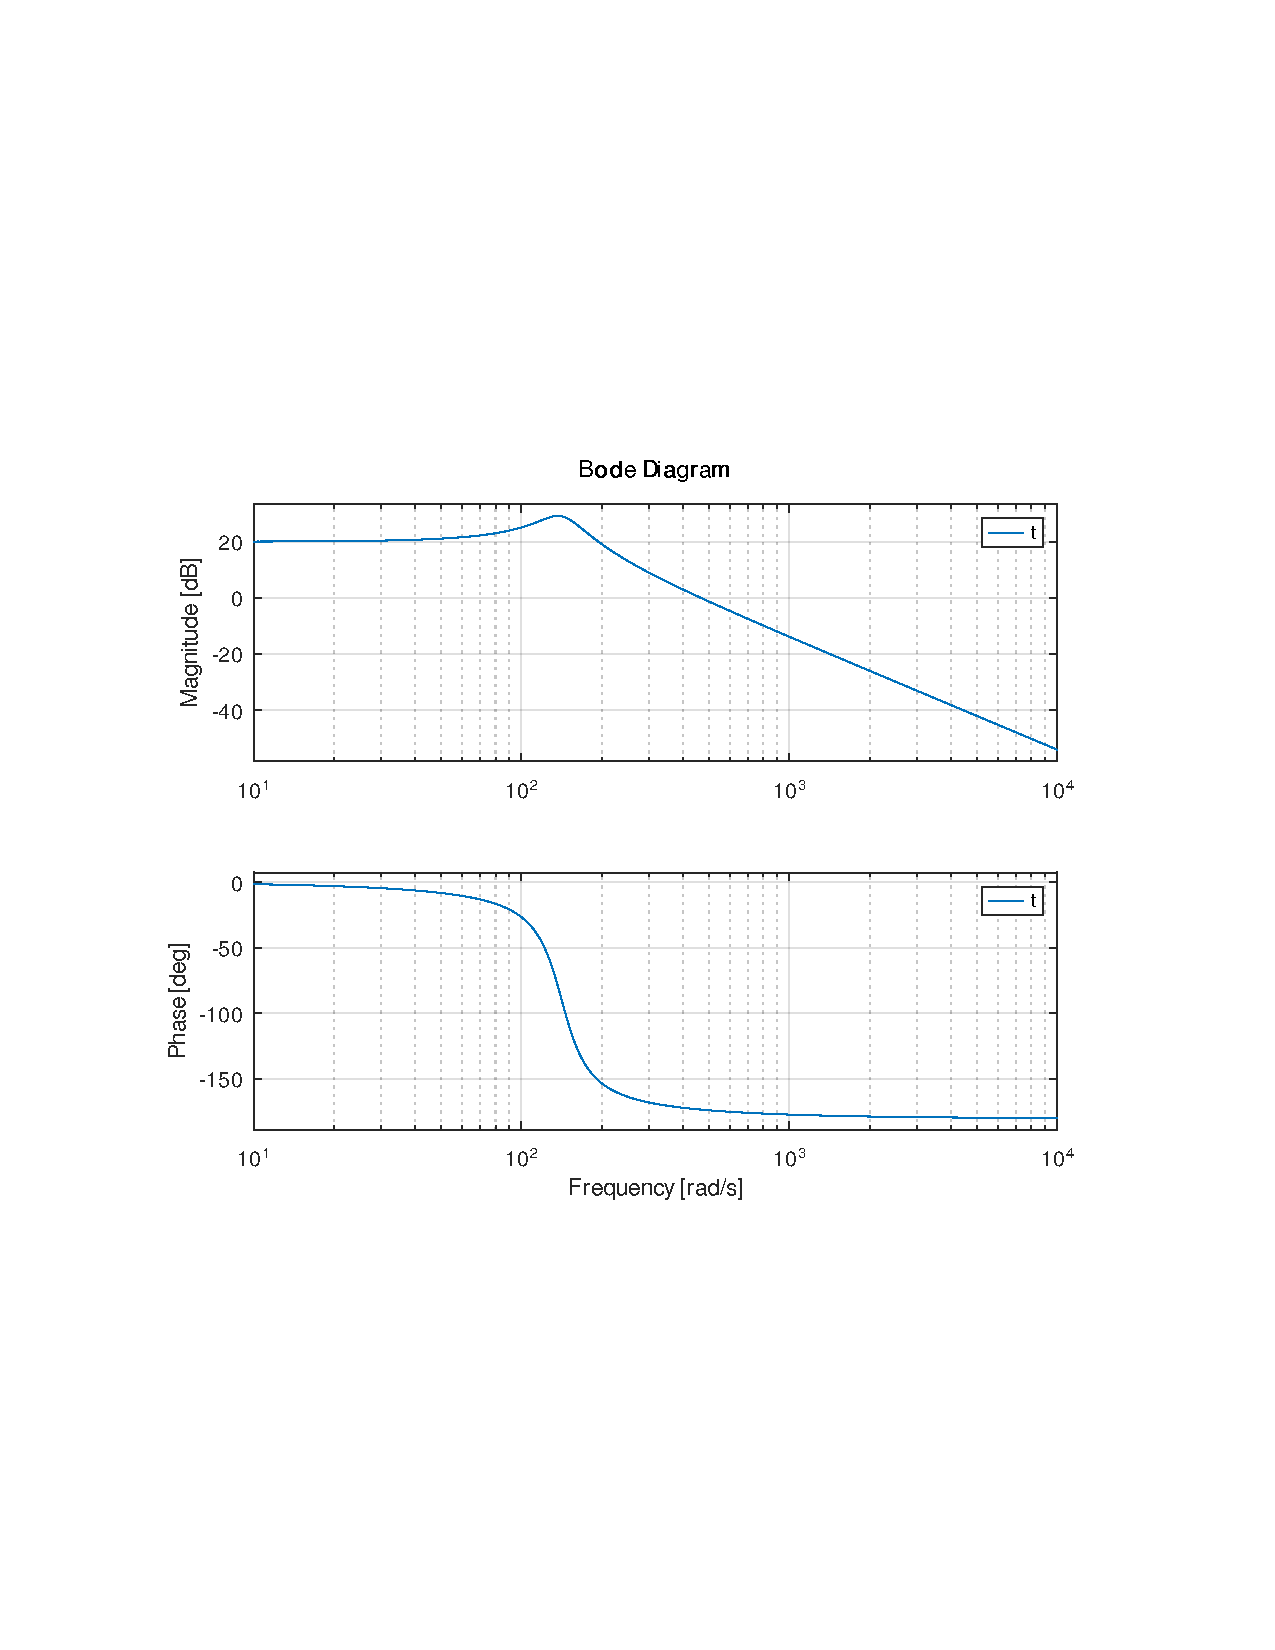
\includegraphics[width=0.6\linewidth,trim={0 7.5cm 0 7.5cm},clip]{figures/bodeplot.pdf}
            \end{figure}
    \end{enumerate}
    \chapter{Practice Exam 2}
    Michael is designing a motor driver for a wheeled mobile robot. The motor driver is designed as
    an inverting amplifier (using the circuit shown in Figure 1) to drive the motor in the opposite
    direction of the input voltage. Michael would like to select the components of the amplifier
    based on specific design requirements. Michael has installed a switch ($Sw_1$) to disconnect the
    motor driver input signal ($v_{in}$) to the system and a motor protection switch ($Sw_2$) to disconnect
    the motor from the amplifier when the motor is not used. A simplified model of a DC motor has
    been used, made up of a resistor and inductor in series. The DC motor generates a torque
    proportional to the current ($i_{out}$) through the inductor
    \begin{figure}[H]
        \centering
        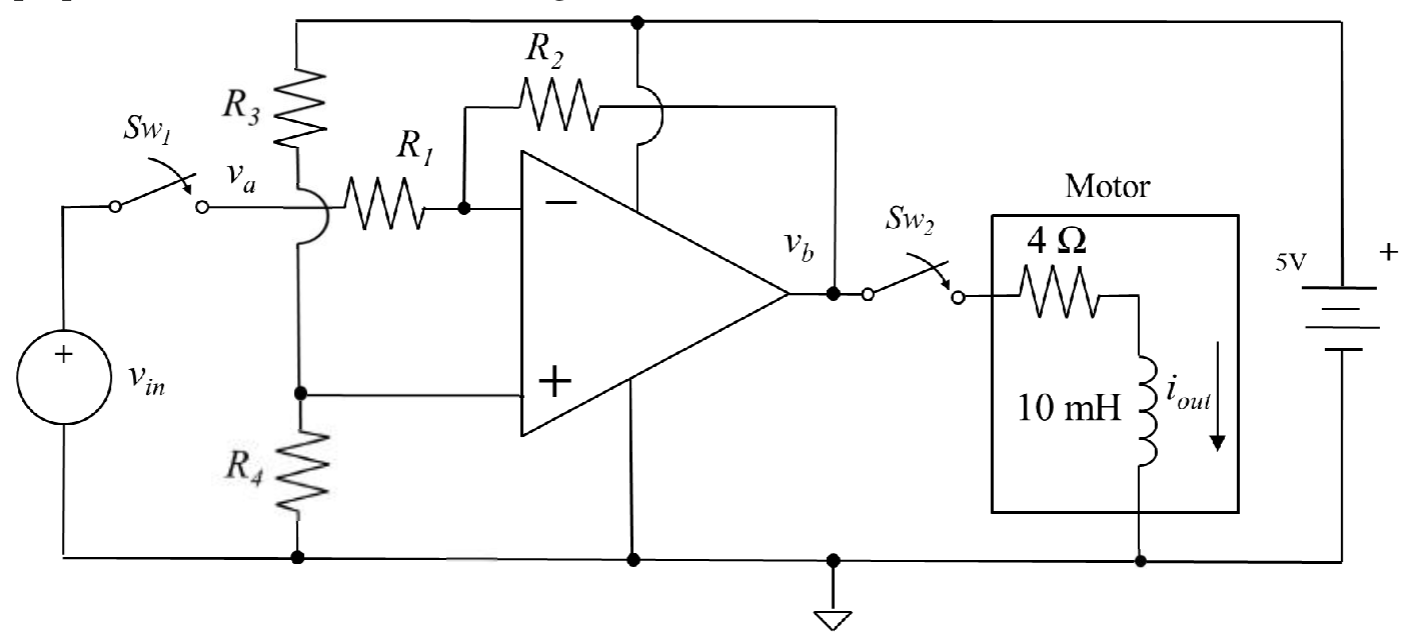
\includegraphics[width=0.6\linewidth]{figures/exams/motor_amp.png}
    \end{figure}
    \begin{enumerate}
        \item Design an inverting amplifier by choosing suitable resistor values for R1 and R2 to
        produce a gain of 5 when both switches Sw1 and Sw2 are open.\\
            \textbf{Solution:}\\
            \begin{minipage}{0.6\linewidth}
                \begin{figure}[H]
                    \centering
                    \begin{circuitikz}[american]
                        % op amp inverting 
                        \draw (0,0) node[op amp] (opamp) {};
                        \draw (opamp.-)
                            to[short, -*] ++(0,1);
                        \draw (opamp.+)
                            to[short, -*] ++(0,-2);
                        % circuit
                    \end{circuitikz}
                \end{figure}
            \end{minipage}
            \begin{minipage}{0.3\linewidth}
                \begin{flalign*}
                    \left|\text{Gain}\right| = \left|-\frac{R_2}{R_1}\right| &= 5\\
                    \text{Let } R_1 &= 1k\Omega\\
                    \therefore R_2 &= 5k\Omega
                \end{flalign*}
            \end{minipage}\\
        \item Design the bias input circuit by choosing suitable resistors R3 and R4 such that the
        voltage $v_b$ will be 0.5V if the positive power supply of the op-amp is connected to a 5V
        battery. Again both switches are open.\\
            \textbf{Solution:}\\
                    \begin{figure}[H]
                        \centering
                        \begin{circuitikz}[american]
                            \draw (0,0)
                                to[resistor, R=R3] (0,2.5)
                                to[resistor, R=R4] (0,5)
                                to[short] (5,5)
                                to[voltage source, v<=5V] (5,1)
                                to[short] (5,0)
                                to[short] (0,0);
                            \draw (2.5,3) node[op amp] (opamp) {};
                            \draw (opamp.up)
                                to[short, -*] ++(0,1.45);
                            \draw (opamp.down)
                                to[short, -*] ++(0,-2.45);
                            \draw (opamp.+) to[short, -*] ++(-1.3,0);
                        \end{circuitikz}
                    \end{figure}    
                    By removing the op amp as its outputs aren't connected we can identify that it is in
                    a voltage divider configuration
                \begin{minipage}{0.6\linewidth}
                    \begin{figure}[H]
                        \centering
                        \begin{circuitikz}[american]
                            \draw (0,0)
                                to[voltage source, v=5V, invert] (0,4)
                                to[short] (2,4)
                                to[resistor, R=R1] (2,2)
                                to[resistor, R=R2] (2,0)
                                to[short] (0,0);
                            \draw (2,2)
                                to[short] (4,2)
                                to[open] (4,0)
                                to[short] (2,0);
                            \node at (4,1) {$v_{out}$};
                            \draw [->] (4,0.8) -- (4,0.1);
                            \draw [->] (4,1.1) -- (4,1.8);
                        \end{circuitikz}
                    \end{figure}
                \end{minipage}
                \begin{minipage}{0.3\linewidth}
                    \begin{flalign*}
                        v_{out} &= \frac{R_2}{R_1 + R_2} v_{in}\\
                        0.5 &= \frac{R_2}{R_1 + R_2} 5\\
                        0.1 &= \frac{R_2}{R_1 + R_2}\\
                        10(R_1 + R_2) &= R_2\\
                        \text{Let } R_1 &= 1k\Omega\\
                        \therefore R_2 &= 9k\Omega
                    \end{flalign*}
                \end{minipage}
        \item Given $Sw_1$ is open, the amplifier is turned on for enough time, such that the voltages
        stabilise, Michael connects the motor by closing Sw2 and the motor starts to move. Find
        the step response of the motor current, iout. Assume that the amplifier output resistance is
        negligible, it does not current limit and the motor inductor has been de-energised\\
            \textbf{Solution:}\\
        \item What is the steady state voltage across the motor?\\
            \textbf{Solution:}\\
        \item Perform frequency response analysis from vin, to the voltage across the motor inductor,
        when both switches are closed and Michael applies three different input signals of 10 Hz,
        100 Hz and 1000 Hz through the system?
            \textbf{Solution:}\\
        \item Plot the response calculated in part (e) in a Bode plot\\
            \textbf{Solution:}\\
    \end{enumerate}
    \chapter{Practice Exam 3}
    Barry the Biologist has asked for your help to build an amplifier and filter to take small signals
    from his bird sensing microphones and amplify them so that he can capture the signals on his
    PC. The microphone produces AC signals at varying frequencies with 10 mV magnitude. His PC
    requires the signals to be 1 V magnitude. The signals that Barry is interested in are above 1 kHz
    Hz. He would like the filter to attenuate signals at frequencies below 1 kHz. The amplifier and
    filter circuit is to be powered from an AC plugpack. The AC plugpack provides 12 VAC RMS at
    50 Hz.
    \begin{figure}[H]
        \centering
        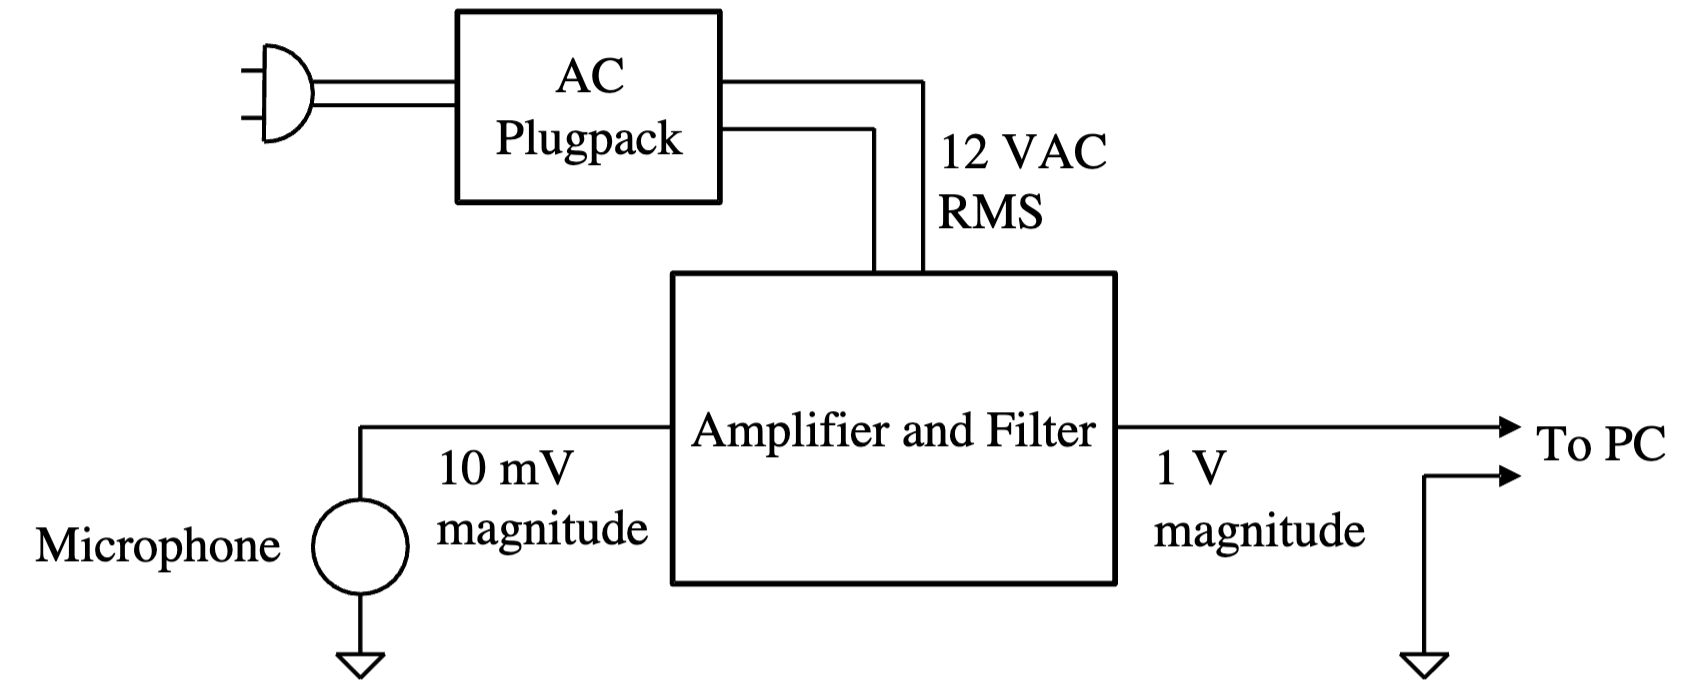
\includegraphics[width=0.6\linewidth]{figures/exams/ac_plugpack.png}
    \end{figure}
    \begin{enumerate}
        \item Design the power supply component of your amplifier and filter. You will need to
        produce a dual-sided power supply with +10V, 0V and -10V using the 12 VAC plug-
        pack as an AC source. Assume that your amplifier and filter will draw around 10 mA of
        current on both the positive and negative voltage supplies. Your design should include
        components to minimise voltage ripple. Show calculations for the selection of
        components where practical. Show a circuit diagram for the complete power supply
        circuit.\\
        \textbf{Solution:}
        In order to minimise voltage ripple, and to have seperate positive and negative voltage components
        we must use 2 half wave rectifiers and a voltage regulator. The voltage regulator will be used to
        regulate the voltage to 10V. The half wave rectifiers will be used to convert the AC voltage to DC.\\
        \textbf{Calculate the capacitance required for the voltage regulator:}
        \begin{flalign*}
            \Delta v = \frac{1}{fC} \Rightarrow C &= \frac{i}{f\Delta v}\\
            \intertext{Using diodes with a forward voltage of 0.7V, with input voltage of 12RMS ($12\sqrt{2}$ VAC) at 50Hz, current of 10mA, and output voltage of 10V:}
            C &= \frac{10\times 10^{-3}}{50\times \left(12\sqrt{2} - 0.7 - (2+10)\right)} \tag{+2 regulated output voltage for linear regulator}\\
            C &= 47\mu \text{F}
        \end{flalign*}
        \textbf{Positive voltage regulator:}
            \begin{figure}[H]
                \centering
                \begin{circuitikz}[american]
                    \draw (8,2) to [short] (8,0);
                    \draw (0,0) 
                    to[sinusoidal voltage source, v<=12V RMS] (0,2)
                    to [diode, l=0.7V] (4,2)
                    to [short] (6,2)
                    to node[rectangle, draw, fill=white] {LM7810} (10,2)
                    to [short] (12,2);
                    \draw (0,0)
                    to [short] (12,0);
                    % components
                    \draw (4,2) to [capacitor, C=47$\mu$F, *-*] (4,0);
                    \draw (6,2) to [capacitor, C=0.33$\mu$F, *-*] (6,0);
                    \draw (10,2) to [capacitor, C=0.1$\mu$F, *-*] (10,0);
                    \node[right] at (12,1) {$v_{out} = 10$ V};
                    % arrow plus minus at 10
                    \draw[->] (12,1.2) -- (12,2);
                    \draw[->] (12,0.8) -- (12,0);
                \end{circuitikz}
            \end{figure}
        \textbf{Negative voltage regulator}
            \begin{figure}[H]
                \centering
                \begin{circuitikz}[american]
                    \draw (8,2) to [short] (8,0);
                    \draw (0,0) 
                    to[sinusoidal voltage source, v<=12V RMS] (0,2)
                    to [diode, l=0.7V, invert] (4,2)
                    to [short] (6,2)
                    to [short] (12,2);
                    \draw (0,0)
                    to [short] (4,0)
                    to [short] (6,0)
                    to node[rectangle, draw, fill=white] {LM7910} (10,0)
                    to [short] (12,0);
                    % components
                    \draw (4,2) to [capacitor, C=47$\mu$F, *-*] (4,0);
                    \draw (6,2) to [capacitor, C=0.33$\mu$F, *-*] (6,0);
                    \draw (10,2) to [capacitor, C=0.1$\mu$F, *-*] (10,0);
                    \node[right] at (12,1) {$v_{out} = -10$ V};
                    % arrow plus minus at 10
                    \draw[->] (12,1.2) -- (12,2);
                    \draw[->] (12,0.8) -- (12,0);
                \end{circuitikz}
            \end{figure}
        \textbf{Half wave rectifier with positive and negative output}
            \begin{figure}[H]
                \centering
                \begin{circuitikz}[american]
                    \draw (8,2) to [short] (8,0);
                    \draw (0,0)
                        to [sinusoidal voltage source, v<=12V RMS] (0,2)
                        to [short, -*] (1,2)
                        to [diode, l=0.7V] (4,2)
                        to [short, -*] (6,2)
                        to node[rectangle, draw, fill=white] {LM7810} (10,2)
                        to [short] (12,2);
                    \draw (0,0)
                        to [short] (12,0);
                    % components
                    \draw (4,2) to [capacitor, C=47$\mu$F, *-*] (4,0);
                    \draw (6,2) to [capacitor, C=0.33$\mu$F, *-*] (6,0);
                    \draw (10,2) to [capacitor, C=0.1$\mu$F, *-*] (10,0);
                    \node[right] at (12,1) {$v_{out} = 10$ V};
                    % arrow plus minus at 10
                    \draw[->] (12,1.2) -- (12,2);
                    \draw[->] (12,0.8) -- (12,0);
                    % negative part
                    \draw (8,0) to [short, -*] (8,-2);
                    \draw (8,-2) to [short, -*] (8,0);
                    \draw (1,-2)
                        to [diode, l=0.7, invert] (4,-2)
                        to [short, -*] (6,-2)
                        to [short] (12,-2);
                    \draw (4,-2)
                        to [short, -*] (4,-2)
                        to [short, -*] (6,-2)
                        to node[rectangle, draw, fill=white] {LM7910} (10,-2)
                        to [short] (12,-2);
                    % components
                    \draw (4,0) to [capacitor, C=47$\mu$F, *-*] (4,-2);
                    \draw (6,0) to [capacitor, C=0.33$\mu$F, *-*] (6,-2);
                    \draw (10,0) to [capacitor, C=0.1$\mu$F, *-*] (10,-2);
                    \node[right] at (12,-1) {$v_{out} = -10$ V};
                    % arrow plus minus at 10
                    \draw[->] (12,-0.8) -- (12,0);
                    \draw[->] (12,-1.2) -- (12,-2);
                    % connect negative part to voltage source
                    \draw (1,-2) to [crossing] (1,2);
                \end{circuitikz}
            \end{figure}
        \item Design the amplifier and filter circuit to meet Barry’s requirements. The circuit must
        produce the required gain, and also attenuate the signals below 1 kHz. Show calculations
        for the selection of components where practical. Show a circuit diagram for the complete
        amplifier and filter circuit. You do not need to redraw the power supply from part (1)\\
        \textbf{Solution:}
        In order to attenuate signals below 1kHz, and allow signals above 1kHz to pass through, we must
        use a high pass filter with a band pass of 1kHz.\\
        As it needs to amplify signals from 10mV to 1V, the gain must be 100.\\
        \textbf{Active High pass filter:}\\
        \begin{minipage}{0.6\linewidth}
            \begin{figure}[H]
                \begin{circuitikz}[american]
                    \draw (0,0) node[op amp] (opamp) {};
                    \draw (-4.5, 0.5) to [capacitor, l_=159nF] ++(1.5,0);
                    \node[above] at (-5,0.7) {$v_{in}$};
                    \draw (-3,0.5) to[resistor, l=$1\text{k}\Omega$] (opamp.-);
                    \draw (opamp.-) to[short] ++(0,1) to[short] ++(0.5,0) to[resistor, l=$100\text{k}\Omega$] ++(3,0) to[short] ++(0,-1.5);
                      \draw (opamp.out) to[short] ++(2,0) node[right] {$v_o$};
                    % ground
                    \draw (opamp.+) to[short] ++(-0.5,0) to[short] ++(0,-0.5) node[ground] {};
                \end{circuitikz}
            \end{figure}
        \end{minipage}
        \begin{minipage}{0.3\linewidth}
            \begin{flalign*}
                \left|\text{Gain}\right| = \left|-\frac{R_2}{R_1}\right| &= 100\\
                \text{Let }R_1 &= 1\text{k}\Omega\\
                \therefore R_2 &= 100\text{k}\Omega\\
                C = \frac{1}{2\pi f R_2} = \frac{1}{2\pi \times 1\text{k}\times 1\text{k}} &= 159\text{nF}\\
            \end{flalign*}
        \end{minipage}
        \item Perform frequency response analysis for the amplifier and filter you designed in part (2)
        to calculate the gain in dB and phase in degrees when the microphone sends a signal at
        100 Hz, 1k Hz and 10 kHz\\
        \textbf{Solution:}
        Using the general form for the transfer function of an active high pass filter:
        \begin{flalign*}
            H(\omega) &= \frac{R_2}{R_1} \frac{j\omega}{j\omega + \frac{1}{R_2C_1}} = 100 \frac{j\omega}{j\omega + \frac{1}{1\times 10^3 \times 159\times 10^{-9}}} = 100\frac{j\omega}{j\omega + 6289.31}
        \end{flalign*}
        \begin{figure}[H]
            \centering
            \begin{tabular}{cccc}
                \textbf{Frequency} & $\boldsymbol{H(\omega)}$ & \textbf{Gain} & $\boldsymbol{\angle H(\omega)}$ \\
                \toprule
                100Hz & $9.947\angle 84.2949^{\circ}$ & 19.948 & 84.2949\\
                1kHz & $70.68\angle 45.03^{\circ}$ & 36.985 & 45.03\\
                10kHz & $99.5\angle 5.72^{\circ}$ & 39.957 & 5.72\\
                \bottomrule
            \end{tabular}
        \end{figure}
        \item Plot the response calculated in part (3) in a Bode plot.\\
            \textbf{Solution:}
            \begin{figure}[H]
                \begin{subfigure}{0.5\textwidth}
                    \centering
                    \begin{tikzpicture}
                        \begin{axis}[
                            xlabel=$x$,
                            ylabel=Phase$(\angle H(\omega))$,
                            domain=1:100000,
                            xmode=log,  % Set x-axis to logarithmic scale
                        ]
            
                        \addplot[blue, smooth, thick] {(atan(-x/6289.31))+90};
                        \end{axis}
                    \end{tikzpicture}
                    \caption{Phase plot}
                \end{subfigure}
                \begin{subfigure}{0.5\textwidth}
                    \centering
                    \begin{tikzpicture}
                        \begin{axis}[
                            xlabel=$x$,
                            ylabel=Gain(dB),
                            domain=1:100000,
                            xmode=log,
                        ]
                        \newcommand{\bodemag}{20*log10(sqrt(100 * x^2 / (x^2 + 6289.31^2)))}
                        \addplot[red, domain=1:100000, samples=1000] {\bodemag};
                        \end{axis}
                    \end{tikzpicture}
                    \caption{Magnitude plot}
                \end{subfigure}
                \caption{Phase and Magnitude plots}
            \end{figure}
    \end{enumerate}
    \chapter{Practice Exam 4}
    Anna the Audiophile has asked for your help to build an amplifier and filter to take small
    signals from her hifi system and amplify them so that she can drive her new subwoofer. The
    hifi system produces AC signals at varying frequencies with 250 mVrms maximum magnitude.
    Her subwoofer requires the signals to be 20 Vrms maximum magnitude. The signals that Anna
    is interested in are below 200 Hz. She would like the filter to attenuate signals at frequencies
    above 200 Hz.
    \begin{figure}[H]
        \centering
        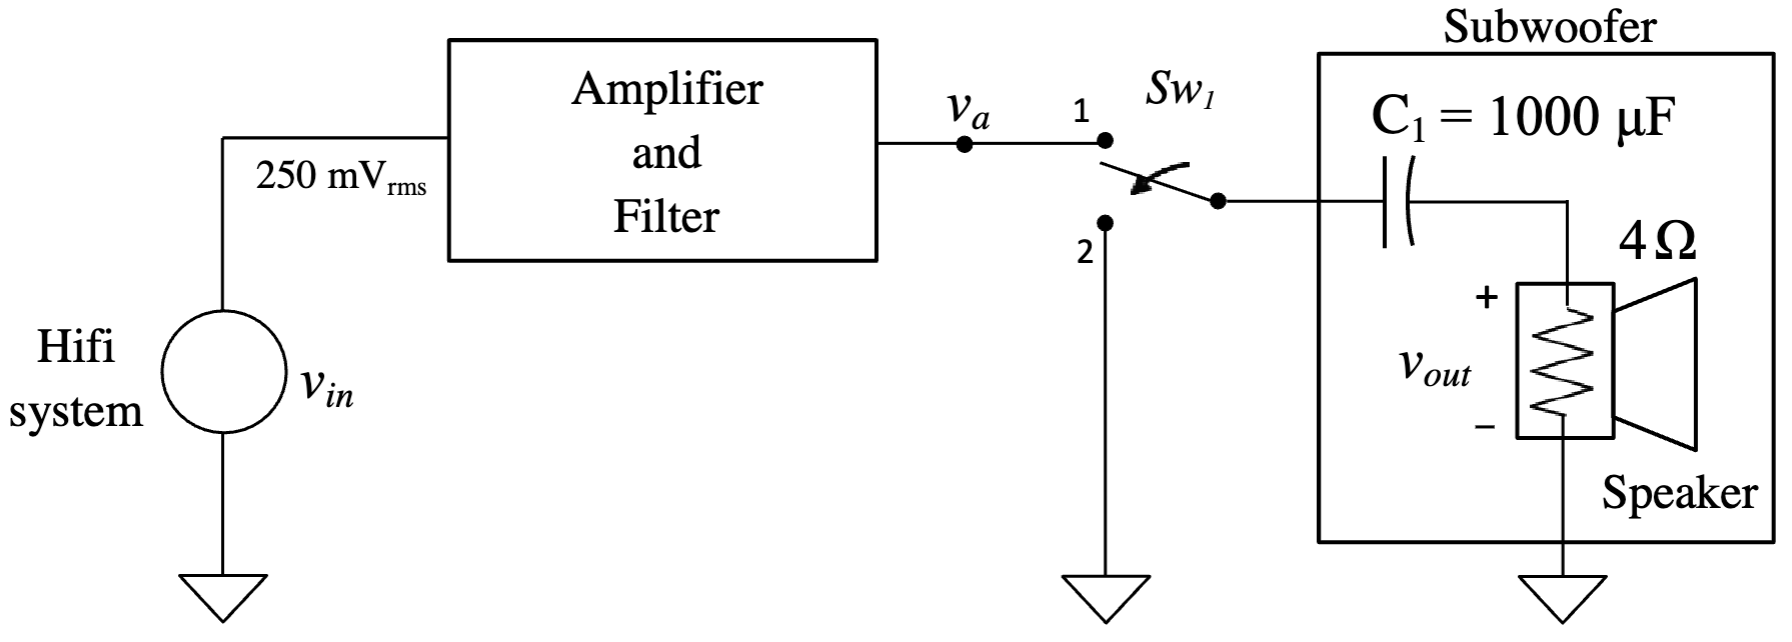
\includegraphics[width=0.6\linewidth]{figures/exams/audiophile.png}
    \end{figure}
    \begin{enumerate}
        \item Design the amplifier and filter circuit to meet Anna’s requirements. The circuit must
        produce the required gain, and also attenuate the signals above 200 Hz. Show
        calculations for the selection of components where practical. Show a circuit diagram for
        the complete amplifier and filter circuit\\
            \textbf{Solution:}\\
            The filter must attenuate all frequencies above 200 Hz. And must increase the gain of the
            input signal. Therefore, an active low-pass filter was chosen.\\
            As it needs to amplify signals from 250 mVrms to 20 Vrms, the gain of the amplifier must be 80.\\
            \begin{minipage}{0.6\linewidth}
                \begin{figure}[H]
                    \centering
                    \begin{circuitikz}[american]
                        \draw (0,0) node[op amp] (opamp) {};
                        \node[above left] at (-3,0.7) {250mV RMS};
                        \draw (-3.5,0.5) to[resistor, R=1k$\Omega$] (opamp.-);
                        \draw (opamp.-) to[short] ++(0,1) to[resistor, R=80k$\Omega$]++(3,0) to[short] ++(0,-1.5);
                        \draw (opamp.-) to[short] ++(0,2.5) to[capacitor, C=10nF] ++(3,0) to[short] ++(0,-3);
                        \draw (opamp.out) to[short] ++(2,0) node[above] {20V RMS};
                        % ground
                        \draw (opamp.+) to[short] ++(-0.5,0) to[short] ++(0,-0.5) node[ground] {};
                    \end{circuitikz}
                \end{figure}
            \end{minipage}
            \begin{minipage}{0.3\linewidth}
                \begin{flalign*}
                    \left|\text{Gain}\right| = \left|-\frac{R_2}{R_1}\right| &= 80\\
                    \text{Let } R_1 &= 1k\Omega\\
                    \therefore R_2 &= 80k\Omega\\
                    C &= \frac{1}{2\pi f R_2}\\
                    &= \frac{1}{2\pi \times 200\times 80\times 10^3}\\
                    &= 10\text{nF}
                \end{flalign*}
            \end{minipage}
        \item Anna reads the subwoofer manual and notes the value of DC blocking capacitor
        C1 = 1000 $\mu$F. She wonders how the capacitor will affect the frequency response of the
        subwoofer. What kind of filter is formed by C1 and the speaker resistance? Calculate the
        cut-off frequency of this filter. Describe the behaviour of this filter in words.\\
            \textbf{Solution:}\\
            The capacitor and the speaker resistance form a high-pass filter with a cut-off frequency 
            defined by
            \begin{align*}
                f_c &= \frac{1}{2\pi R C}\\
                &= \frac{1}{4\times 1000\times 10^{-6}\times 2\pi}\\
                &= 40\text{Hz}
            \end{align*}
            This filter will attenuate all frequencies below 40 Hz.
        \item When first turned on, Anna’s amplifier fails and applies +15V DC directly to the output
        (va). After 30 milliseconds, the speaker protection circuit operates Sw1 to disconnect the
        speaker and connect it to ground (Sw1 changes from position ‘1’ to position ‘2’). Taking
        the time the amplifier was turned on as t=0 seconds, calculate and plot the voltage across
        the speaker for the first 60 milliseconds. Ensure your drawing is to scale and has labelled
        key values\\
            \textbf{Solution:}\\
            First isolate the circuit at $t=0$.\\
            \begin{minipage}{0.6\linewidth}
                \begin{figure}[H]
                    \centering
                    \begin{circuitikz}[american]
                        \draw (0,0) 
                            to[voltage source, invert, v=15V] (0,2)
                            to[capacitor, l=1000$\mu F$] (2,2)
                            to[resistor, R=4$\Omega$] (2,0)
                            to[short] (0,0); 
                    \end{circuitikz}
                \end{figure}
                Apply source transformation from Thevenin to Norton equivalent\\($I = \frac{V}{R} = \frac{15}{4} = 3.75A$)
                \begin{figure}[H]
                    \centering
                    \begin{circuitikz}[american]
                        \draw (0,0)
                            to[current source, i=3.75A] (0,2)
                            to[short] (4,2)
                            to[capacitor, l=1000$\mu$F] (4,0)
                            to[short] (0,0);
                        \draw (2,0) to[resistor, R=4$\Omega$] (2,2);
                    \end{circuitikz}
                \end{figure}
                \begin{figure}[H]
                    \centering
                    \begin{tikzpicture}
                        \begin{axis}[
                            xlabel=$t$,
                            ylabel=$v$,
                            legend style={nodes={scale=0.8, transform shape}},
                        ]
                        \addplot[blue, domain=0:0.03] {15 - 15*exp(-250*x)};
                        \addplot[red, domain=0.03:0.06] {14.9917*exp(-250*(x-0.03))};
                        \legend{Step response, Natural response}
                        \end{axis}
                    \end{tikzpicture}
                    \caption{Voltage across the speaker}
                \end{figure}
            \end{minipage}
            \begin{minipage}{0.4\linewidth}
                For step response ($0<t<0.03$) (capacitor charging)
                \begin{flalign*}
                    v(t) &= I_s R + (V_o - I_s R)e^{-\frac{t}{RC}}\\
                    &= 3.75\times 4 + (0 - 3.75\times 4)e^{-\frac{t}{100\times 10^{-6}\times 4}}\\
                    &= 15 - 15e^{-250t}\\
                    v(0.03) &= 15 - 15e^{-250\times 0.03} = 14.9917\\
                    \intertext{For natural response ($t>0.03$) (capacitor discharging), $V_o = 14.9917$}
                    v(t) &= V_o e^{-\frac{t-0.03}{RC}}\\
                    &= 14.9917e^{-250(t-0.03)}\\\\\\\\\\\\\\\\\\\\\\\\\\\\\\
                \end{flalign*}
            \end{minipage}\\
        \item The amplifier fault has now been fixed and the system works normally (Sw1 is in
        position ‘1’). Perform frequency response analysis for the amplifier and filter you
        designed in part (a) to calculate the gain in dB and phase in degrees when the hifi system
        sends a signal at 10 Hz, 100 Hz and 1000 Hz.\\
            \textbf{Solution:}\\
            \begin{flalign*}
                H(\omega) &= -\frac{R_2}{R_1} \frac{\frac{1}{R_2 C}}{j\omega + \frac{1}{R_2 C}} \tag{$\frac{1}{R_2C} = \frac{1}{80\times 10^{3}\times10^{-9}} = 1250$}\\
                &= -80\frac{1250}{j\omega + 1250}
            \end{flalign*}
            \begin{figure}[H]
                \centering
                \begin{tabular}{cccc}
                    $\boldsymbol{\omega}$ & $\textbf{H}(\boldsymbol{\omega})$ & $\textbf{Gain (dB)}$ & $\textbf{Phase (degrees)}$\\
                    \toprule
                    $20\pi$ & $79.899\angle 177.122^{\circ}$ & 38.051 & 177.122\\
                    $200\pi$ & $71.4781\angle 153.313^{\circ}$ & 37.084 & 153.313\\
                    $2000\pi$ & $15.6096\angle 101.252^{\circ}$ & 23.868 & 101.252\\
                    \bottomrule
                \end{tabular}
                \caption{Frequency response analysis}
            \end{figure}
        \item Calculate the output voltage of the amplifier and filter circuit (va) when a 250 mVrms,
        100 Hz signal is applied at its input ($v_{in}$)\\
            \textbf{Solution:}
            \begin{flalign*}
                V_{out} &= V_{in}H(\omega)\\
                &= 0.25\times\sqrt{2} \times H(200\pi)\\
                &= 0.25\times\sqrt{2} \times 71.4781\angle 153.313^{\circ} \tag{From part (d)}\\
                &= 25.2713\angle 153.313^{\circ}
            \end{flalign*}
    \end{enumerate}
\end{document}